\chapter{Tandem mass spectrometry in the context of disulfide bond analysis}

In the introduction we have established that disulfide bonds (DB) are important to protein function, structure, and to enzyme regulation. We have also shown that information about their positions can be used to optimise folding methods that are based on molecular dynamic simulations. We hope that these are enough to persuade the reader that studying the DB positions in a protein is a worthwhile task, although a complicated one.

There are many methods aiming to determine the positions of DBs; the most popular is tandem mass spectrometry (MS/MS). MS/MS is a popular analysis technique, often used in proteomics, and specifically DB mapping, for its accuracy, sensitivity and speed.~\cite{gorman2002protein}

In MS/MS analysis (or more accurately its bottom-up variant), the protein is eventually fragmented to smaller charged peptides whose mass to charge ratio (\(m/z\)) is measured with atomic precision. Multiple sets of \emph{fragmentation spectra} are obtained, each coming from a longer peptide with a specific \(m/z\) value that is called the \emph{precursor}. While in proteomics the task is usually to identify the original protein from the fragments, during DB mapping it is known which protein the fragments come from, and instead the task is to determine the positions of its DBs.

The experiment can be designed in a way that keeps the DBs intact, resulting in the occurence of crosslinked peptides with specific fragmentation signatures. There are multiple analytical methods, both manual and computational, that try to discover these fragmentation spectra and use them to determine the positions of the DBs in the protein. Other methods choose to dissociate the DBs during the fragmentation, a process that leads to another kind of specific fragmentation signatures.

The first few sections of this chapter roughly reflect the first few steps in a mass spectrometry experiment.

\begin{enumerate}
  \item The first topic we discuss is sample preparation, an important prerequisite in bottom-up mass spectrometric analysis (\Cref{sec:trypsin}).
  \item In \Cref{sec:lc}, a short overview of sample separation methods is provided.
  \item With the sample being digested and separated, we move on to explain the principles behind mass spectrometry itself, putting the focus on methods and techniques that are relevant to disulfide bond analysis (\Cref{sec:msms}). Where possible, we compare multiple methods and state their tradeoffs in the context of our work.
  \item Finally, we list some of the current approaches to DB mapping, noting their respective strengths and weaknesses (\Cref{sec:analysis}). At the very end of this chapter, we reformulate the task in more formal terms and roughly approximate its computational complexity.
\end{enumerate}

\section{Protein digestion and sample preparation}\label{sec:trypsin}

In order for the protein to be analysed, it first needs to be digested into smaller peptides; trypsin, and, to a lesser extent, pepsin, are popular choices in general proteomics.

Trypsin is a serine protease that cleaves amino acid chains at the carboxyllic side of lysine and arginine, provided they are not followed by proline~\cite{olsen2004trypsin}. Lysine and arginine are both relatively abundant in most proteins which makes the tryptic digestion peptides --- or as we will call them, \emph{tryptides} --- reasonably sized for a mass spectrometry analysis~\cite{matthiesen2020trypticsize}. Additionally, trypsin has very high specificity, and thus the digestion peptides are quite predictable. That being said, the sample protein is not cleaved at every potential cleavage site; so called \emph{missed cleavages} do occur during most proteolytic digestions. The frequency of missed cleavages depends on neigbouring residues of the cleavage site~\cite{gershon2014cleaved}, the used protease, and the experimental setup.

Relevant to our work is the following particularity of trypsin and some other proteases: they require a neutral-to-basic environment in order to become proteolytically active. In this environment the issue of DB scrambling arises~\cite{wu1997novel}; some of the DBs become dissociated, then the cysteines re-connect, but in different patterns than before. These scrambled bonds are diffucult to discern from the naturally occuring ones in the mass spectra. The issue can be mitigated by using a different protease for the digestion, such as pepsin, or thermolysin~\cite{sung2016evaluation}.

In addition to digestion, in a general proteomic experiment the protein usually undergoes reduction that completely dissociates the DBs, and cysteine alkylation that prevents the cysteines from reassociating. However, in an experiment that aims to characterise cysteine linkages, only the alkylation is performed, and the present DBs are kept intact.

\section{Liquid chromatography sample separation}\label{sec:lc}

In a general proteomic experiment, the signal from more abundant sample peptides may interfere with the other, less frequent ones. To sidestep this problem, it has become routine to perform separation before the main MS experiment, either on the protein level or the peptide level. After separation, less analytes are present in a mass spectrometer at a given point in time, reducing the chance of a signal becoming lost. Protein-level separation is common among experiments with the goal of identifying which proteins are present in the sample; in the case of disulfide bond characterisation, there is only one protein present, so peptide-level separation is the method of choice.

A popular peptide-level separation method is liquid chromatography (LC). In a model proteomic MS-LC experiment, the proteins are digested without prior separation, and the resulting peptides are separated on reverse-phase liquid chromatography column that is directly connected to a tandem mass spectrometer~\cite{washburn2001large}. This process is applicable to DB analysis as well.

Reverse-phase LC has two main constituents: a mobile liquid phase that contains the peptides, and a stationary solid phase which is usually a nonpolar column with \(\ce{C18}\) alkyl chains~\cite{chang1976high}. The mobile phase passes along the stationary phase, the elution time of each individual peptide depending on its hydrophobic interactions with the alkyls. The peptides are eluted with a polar mixture of water and organic solvent, such as acetonitrile~\cite{frohlich2006proteome}, the shortest and least hydrophilic peptides eluting the earliest.

The LC column is often directly connected to the mass spectrometer, which performs the bulk of the analysis.


\section{Tandem mass spectrometry}\label{sec:msms}

Mass spectrometry is an analytical technique that has originally been used for studying small thermostable molecules. Nevertheless, with the advancements in soft ionization allowing proteins and other biomolecules to be analysed as well~\cite{fenn1989electrospray}, mass spectrometry has become an indispesable tool in proteomics research~\cite{collins2003human}.

Mass spectrometry experiments can be either single-stage (MS) or tandem, the latter being denominated MS/MS, sometimes MS\textsuperscript{2}, and in the cases of more than two subsequent analyses, MS\textsuperscript{\(n\)}. During single-stage experiments, the mass distribution of a polypeptide sample is determined. The more frequent of the two, tandem mass spectrometry is used to learn about certain structural features of a protein, including sequence and post-translational modifications.~\cite{domon2006mass}

\begin{figure}
  \centering
  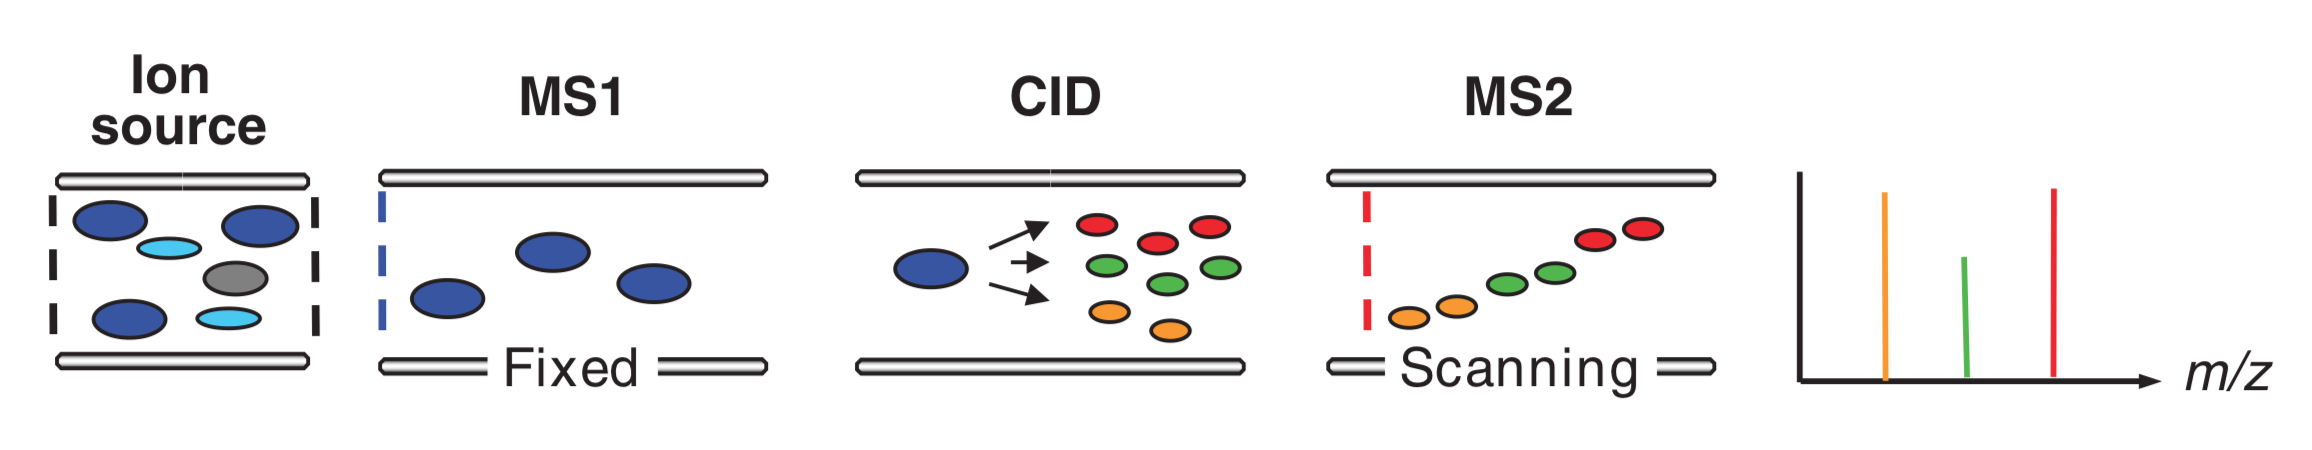
\includegraphics[width=.9\linewidth]{img/msms-workflow.png}
  \caption{A diagram of an ordinary MS/MS workflow. While the specific instrumentation details differ from spectrometer to spectrometer, the general structure of ionize \textrightarrow{} analyse \textrightarrow{} fragment \textrightarrow{} analyse is common to all MS/MS experiments. Image by~\citet{domon2006mass}.}\label{fig:mass-spectrometry-workflow}
\end{figure}

Both the single-stage and MS/MS experiments begin similarly: the sample peptides are ionized (see \Cref{sec:ionisation}), and the ions travel through an electromagnetic field in an analyser whilst their mass-to-charge (\(m/z\)) is being calculated (\Cref{sec:msms-analysis})~\cite{gross2006mass}. In single-stage mass spectrometry, the experiment ends there, while in MS/MS, some of these \emph{precursors} are selected to undergo fragmentation in the collision cell (\Cref{sec:fragmentation}); the typical MS/MS workflow is shown on \Cref{fig:mass-spectrometry-workflow}. The resulting fragments are analysed and their \(m/z\) values noted; the output of the MS/MS experiment is made of precursors with their masses and their fragmentation spectra; an example of a precursor fragmentation spectrum can be seen on figure \Cref{fig:frag-spectrum}.

\begin{figure}
  \centering
  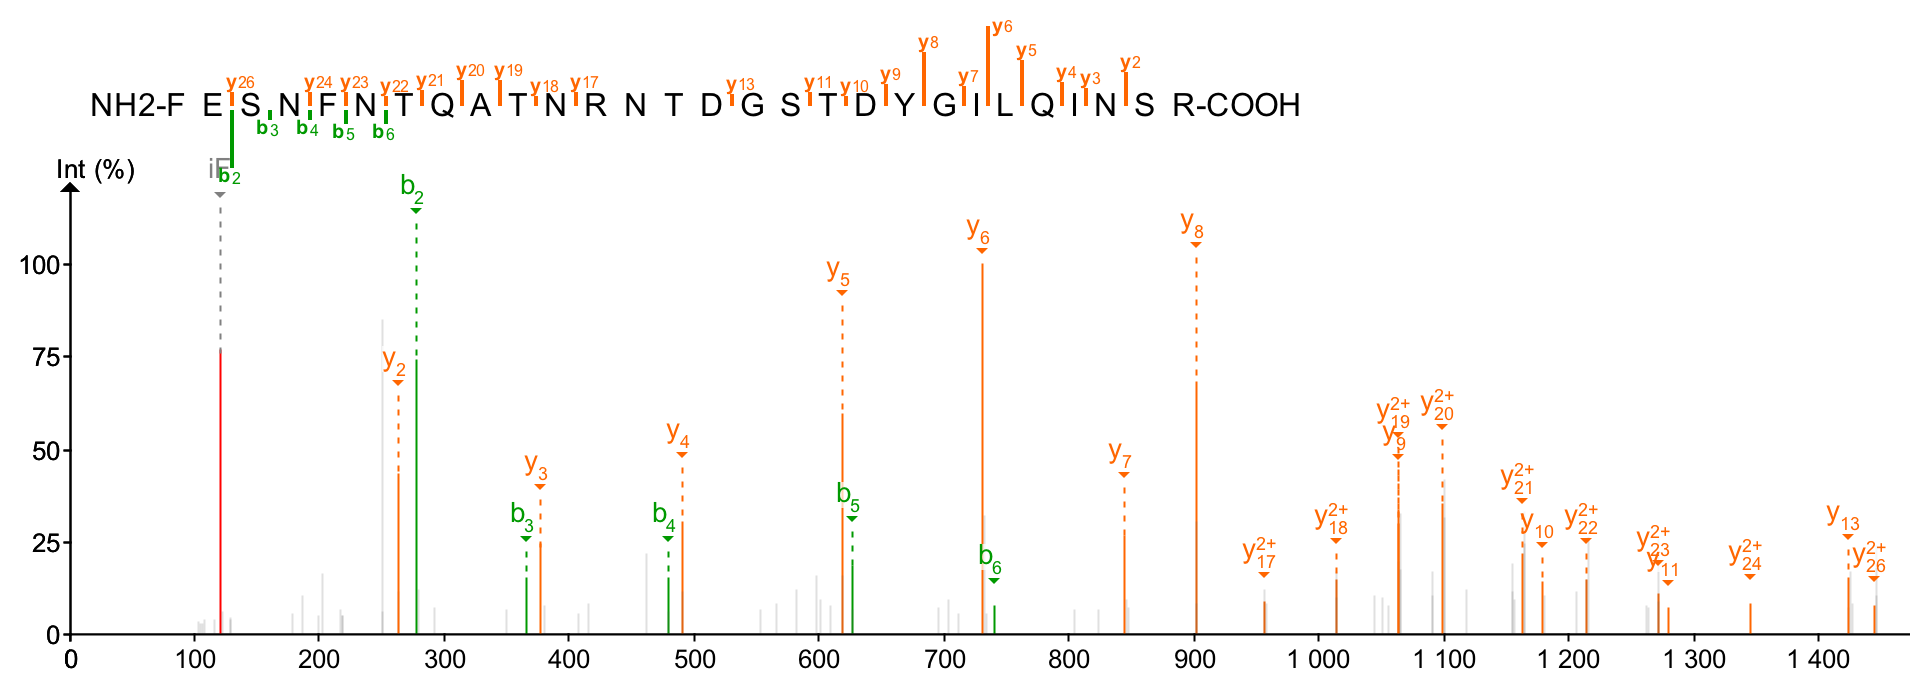
\includegraphics[width=1\linewidth]{img/fragmentation-spectrum.png}
  \caption{An annotated fragmentation spectrum of the precursor \emph{FESNFNTQATNRNTDGSTDYGILQINSR}. A \emph{peak} signifies that a peptide with a specific \(m/z\) value has been seen, and also provides information about the intensity of its signal.}\label{fig:frag-spectrum}
\end{figure}

When the analysed protein is crosslinked by DBs, some of the precursors will be crosslinked, too. The aim of the DB MS/MS analysis is to identify the crosslinked precursors and deduce the positions of DBs in the protein. Specific instrumentation choices influence the behaviour of crosslinked peptides during the analysis, and result in fragmentation spectra with vastly different characteristics. Sometimes one approach is preferable; for example in the case of picking an analyser, orbitrap is usually preferred thanks to its accuracy and sensitivity. Other times the choice is more ambiguous, such as the choice between CID and ETD fragmentation. We discuss the possible intstrumentation choices in the context of DB mapping in the following sections; the overview is partly based on the works of \citet{matthiesen2007mass} and \citet{gross2006mass}.

\subsection{Sample ionization}\label{sec:ionisation}

Only charged compounds in gas phase are detectable by a mass spectrometer analyser. If the samples are not in this form, they need to be ionised.

One of the oldest ionisation methods is electron ionization (EI)~\cite{field2013electron}. However, EI is unsuitable for large thermally unstable organic molecules, such as peptides; for proteomics work, the two most popular options are MALDI and ESI~\cite{caprioli1997molecular, fenn1990electrospray}.\@ Unlike ESI, the MALDI ionisation process has to be done in a vacuum, making it impossible to directly connect a LC column to the spectrometer. Thus, for the purpose of DB mapping, ESI is usually the ionisation method of choice.

During ESI, a very fine capillary with a solution that contains the sample peptides and charged ions is placed into a strong electrostatic field. Due to the influence of the field, the solution forcibly squirts out of the capillary, creating a mist of miniscule charged droplets. The solution slowly evaporates from the droplets, until eventually the repulsive electric forces inside the droplet overcome its surface tension and the droplet splits into yet smaller droplets~\cite{rayleigh1882xx}. This evaporating and splitting process repeats itself, until we are left with isolated sample ions in the gas phase~\cite{dole1968molecular,dole1968gas,fenn1989electrospray, fenn1990electrospray}.

For our work, three properties of ESI are important.

\begin{itemize}
  \item ESI works under atmospheric pressure, enabling the LC colon to be connected directly to the mass spectrometer, creating an ``online'' or ``hyphenated'' LC-MS system~\cite{opiteck1997comprehensive}. This property simplifies the MS/MS experiment and provides higher throughput.
  \item The ionisation cases very little to no fragmentation to the sample~\cite{griffiths2001electrospray} --- in other words, ESI a ``soft'' ionisation technique. This property is useful because it simplifies the subsequent analysis, and does not add noise to the measured information.
  \item  Ions generated by ESI are often multiply charged~\cite{felitsyn2002origin}, bringing their \(m/z\) value down and enabling us to analyse peptides with a higher mass in an ordinary mass spectrometer setting.
\end{itemize}

\subsection{Mass analysers}\label{sec:msms-analysis}

A mass analyser, sometimes equipped with a separate detector, measures the mass to charge ratio (\(m/z\)) and intensity of a sample compound. The many existing mass analysers differ in the principle of function, and their performance characteristics.

\begin{description}
  \item[Time-of-flight analyser] In TOF analysers~\cite{stephens1946pulsed}, sample ions are accelerated with an electric field to make them travel along a path with known length. The ions with lower \(m/z\) values will arrive measurably sooner than the ones with higher \(m/z\) values, as long as all of them are dispersed at a similar-enough points in time. Due to this requirement, TOF analysers are best suited for pulsed ionization techniques such as MALDI\@. TOF analysers have an excellent sensitivity and, at least in theory, their \(m/z\) range is unlimited~\cite{fuerstenau1995molecular}.
  \item[Linear quadrupole analyser] As the name suggest, a linear quadrupole consist of four linear rods which are placed parallel to each other and arranged in a square shape, see \Cref*{fig:quadrupole}. A pair of rods sitting in diagonally opposite corners has the same polarity, however, the pairs periodically switch the polarity. An ion travelling along the rods is periodically repelled and attracted to each of the rods, its precise trajectory depending on its \(m/z\) value~\cite{paul1990electromagnetic}. In this way, ions with specific \(m/z\) values can pass through the quadrupole into a detector~\cite{paul1953neues}, while others follow an unstable trajectory and crash into one of the poles or the wall of the quadrupole.

    Quadrupoles can also trap specific ions inside instead of making them simply pass through; such quadrupole is usually called a linear ion trap~\cite{mao2003h}. Furhtermore, quadrupoles can serve as fragmentation collision cells. Due to their flxibility, a tripple-quadrupole mass spectrometer was a popular choice for MS/MS experiments~\cite{yost1978selected}.
  \item[FT-ICR analyser] In Fourier transform ion cyclotron resonance analysers (FT-ICR) the analytes circulate in a magnetic field, and Fourier transform is used to decode the induced signals. The \(m/z\) values are calculated from the frequencies and amplitudes~\cite{comisarow1974fourier}. Many ions with wildly different \(m/z\) values can be measured in parallel, making the analysis faster. Further improvements also increased the mass accuracy and resolution beyond what is attainable by quadrupole analysers~\cite{amster1996fourier, easterling1999routine}.
  \item[Orbitrap analyser] The Orbitrap is the most imporant analyser type in the context of our work~\cite{hu2005orbitrap}. It achieves similar accuracy, resolving power, and dynamic range to FT-ICR, but does not require an expensive-to-run supraconducting magnet to do so. In Orbitrap the ions simultaneously cycle around the centre and oscillate along the z-axis, as is illustrated on \Cref*{fig:orbitrap}. This oscillation induces a periodically changing electrical current in the detector that is converted to a \(m/z\) spectrum of the analyte with the help of Fourier transform.

    The Orbitrap often achieves sub-ppm error rates, which makes it ideal for our usecase. Our goal is to identify complicated ions, and for that we need the measurements of their mass to be as reliable as possible. Furthermore it is possible to connect Orbitrap to an ESI ion source, and by extension to a LC colon.
\end{description}

\begin{figure}
  \centering
  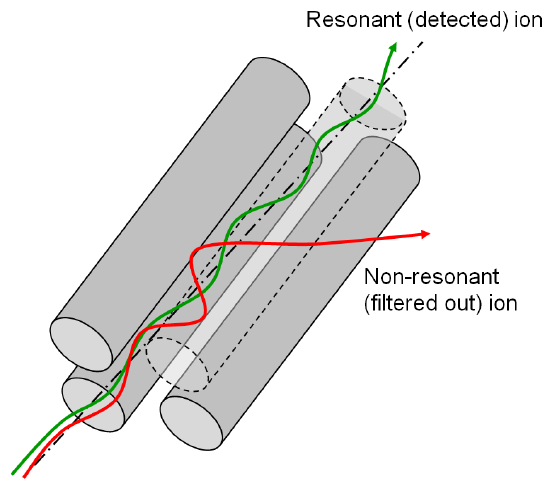
\includegraphics[width=.4\linewidth]{img/quadrupole.png}
  \caption{A quadrupole with two highlighted classes of ion trajectories. Thanks to its \(m/z\) value, the ion with green trajectory passes through the quadrupole and is ultimately detected, while the one with the red trajectory is filtered out. Image taken from~\citet{2021Mass}.}\label{fig:quadrupole}
\end{figure}

\begin{figure}
  \centering
  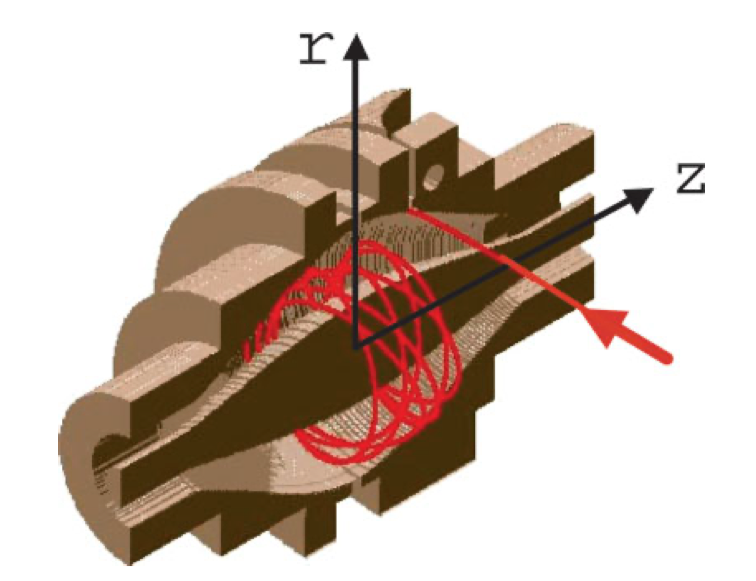
\includegraphics[width=.5\linewidth]{img/orbitrap.png}
  \caption{An Orbitrap mass analyser with a typical ion trajetrory highlighted. The ion circulates around the center while simultanously oscillating along the z-axis. Image by~\citet{hu2005orbitrap}.}\label{fig:orbitrap}
\end{figure}

\subsection{Precursor fragmentation}\label{sec:fragmentation}

In MS/MS experiments, once the mass spectrum of the initial sample is analysed and the MS\textsuperscript{1} data are acquired, \emph{precursors} are selected according to their mass, and fragmented. The fragments undergo yet another mass analysis, producing so called MS\textsuperscript{2} data. In the section we present a short overview of the currently used fragmentation methods.

When the goal of the experiment is to observe post-translational modifications (PTMs) and to preserve the volatile bond connecting the PTM to the peptide, electron-capture dissociation (ECD)~\cite{zubarev2000electron} or electron-transfer dissociation (ETM)~\cite{syka2004peptide} are preferred. Both methods use electron transfer to induce amine backbone bond cleavage that results in the creation of \(c\) and \(z\) ions, as illustrated on \Cref{fig:fragment-types}.

During ETD, the DBs are dissociated, and the crosslinked precursor is split into its constituent peptides~\cite{liu2014facilitating}. These peptides appear as high-intensity peaks in the fragmentation spectra. The peaks which can be used to determine the peptide makeup of the orignal precursor, which causes ETD to be a popular fragmentation technique in DB mapping methods. However, if the precursor contains multiple cysteines, it may be hard to deduce which of them were paired together, especially if there were multiple DBs present. In this work we focus on methods that do not have this disadvantage.

First of these methods is collision-induced dissociation (CID). CID accelerates the precursor ions, and makes them collide with neutral gas molecules, ultimately leading to their fragmentation. The dissociation process usually takes place at the more labile bonds, such as the ones connecting PTMs~\cite{quan2013cid}, or peptide bonds in the precursor backbone.\footnote{The fact that many PTM bonds are preferentially dissociated during CID is usually seen as unfortunate. However, in the case of DB mapping it simplifies the analysis, as the PTMs can be safely ignored, which reduces the combinatorial complexity of the problem.} CID produces \(b\) and \(y\) fragment ions (see \Cref{fig:fragment-types}); additionally, as a side-effect of the dissociation, a small neutral molecule sometimes breaks off of the fragment, lowering its total mass value without affecting its charge. This dissociated molecule is called a \emph{neutral loss}. In CID, the most common neutral losses are water and amonia.

A specific variant of CID called the beam-type CID produces \emph{internal ions}, fragments that are generated by two (or more) bond cleavages during the fragmentation. Many of the internal ions begin with a proline~\cite{michalski2012systematic}, suggesting that the double cleavage event prefers some amino acids to others. As shown by \citet{michalski2012systematic}, ion-trap CID, the other CID variant, does not produce internal ions. Furthermore, ion-trap CID has limits regarding the containment of molecules below a certain mass threshold, leading to a mass cutoff~\cite{louris1987instrumentation}.

\begin{figure}
  \centering
  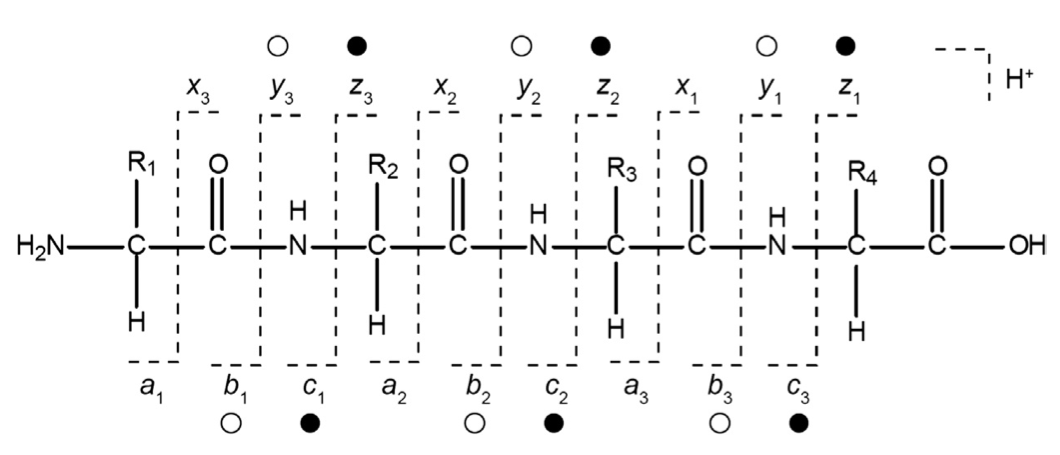
\includegraphics[width=.75\linewidth]{img/fragment-types.png}
  \caption{A singly positively charged peptide with annotated fragmentation types. Signature CID b/y ion fragments are marked with open circles, while the typical ECD and ETD c/z ion fragments are marked with filled circles. Image by~\citet{hart2014review}.}\label{fig:fragment-types}
\end{figure}

A similar fragmentation signature to CID can also be obtained by infrared multiphoton dissociation (IRMPD)~\cite{oomens2006gas}. Because IRMPD, and the related UV-MPD, do not require collision gasses to be present for the fragmentaion, they are well suited for analysers operating under high vacuum, such as FT-ICR\@.

In 2007 a new fragmentation method based on beam-type CID has been devised, called the higher-energy C-trap dissociation (HCD)\@. The fragmentation spectra obtained from CID and HCD are very similar~\cite{michalski2012systematic}, nonetheless there is a key difference between the two methods: HCD combines the richer sequence information~\cite{xia2006ion} and lower mass cutoff of beam-type CID with the superior resolution capacity and accuracy of the orbitrap analyser. That is one of the reasons the data we use in this thesis come from HCD\@. In the next section we describe the common HCD fragmentation pathways, because they are crucial to the function of our DB mapping program.

\subsubsection{Fragmentation pathways in HCD}

Fragments from ESI-ionized precursors can be and indeed often are multiply charged~\cite{katta1991use, michalski2012systematic}. According to the research on CID of crosslinked peptides by \citet{giese2016study}, most of the crosslinked fragments were found to have a positive charge of at least 2, while an overwhelming majority of linear fragments had a positive charge of 1. HCD is in principle similar to CID, and we believe these findings woud translate to HCD-generated fragments as well.

The different types of fragments of a very pure sample were nicely summarized by \citet{michalski2012systematic}. Ions of \(b\), \(y\) and \(a\) type comprise most of the spectral intensity (54\%, see \Cref{fig:hcd}). The ions themselves have different distributions, the \(y\) type being the most abundant. Other neutral loss ions, be it a loss of water, amonia, or an amino-acid-specific small molecule\footnote{If specific amino acid neutral losses are of interest, the review by~\citet{paizs2005fragmentation} lists many of them.}, together with internal ions, can be attributed a quarter of the total fragment intensity. Finally, immonium ions account for 6\% of the intensity. In total 85\% of the spectral intensity is explainable. For a visual overview of the many different HCD fragmentation types, please refer to \Cref{fig:fragment-types-hcd}.

\begin{figure}
  \centering
  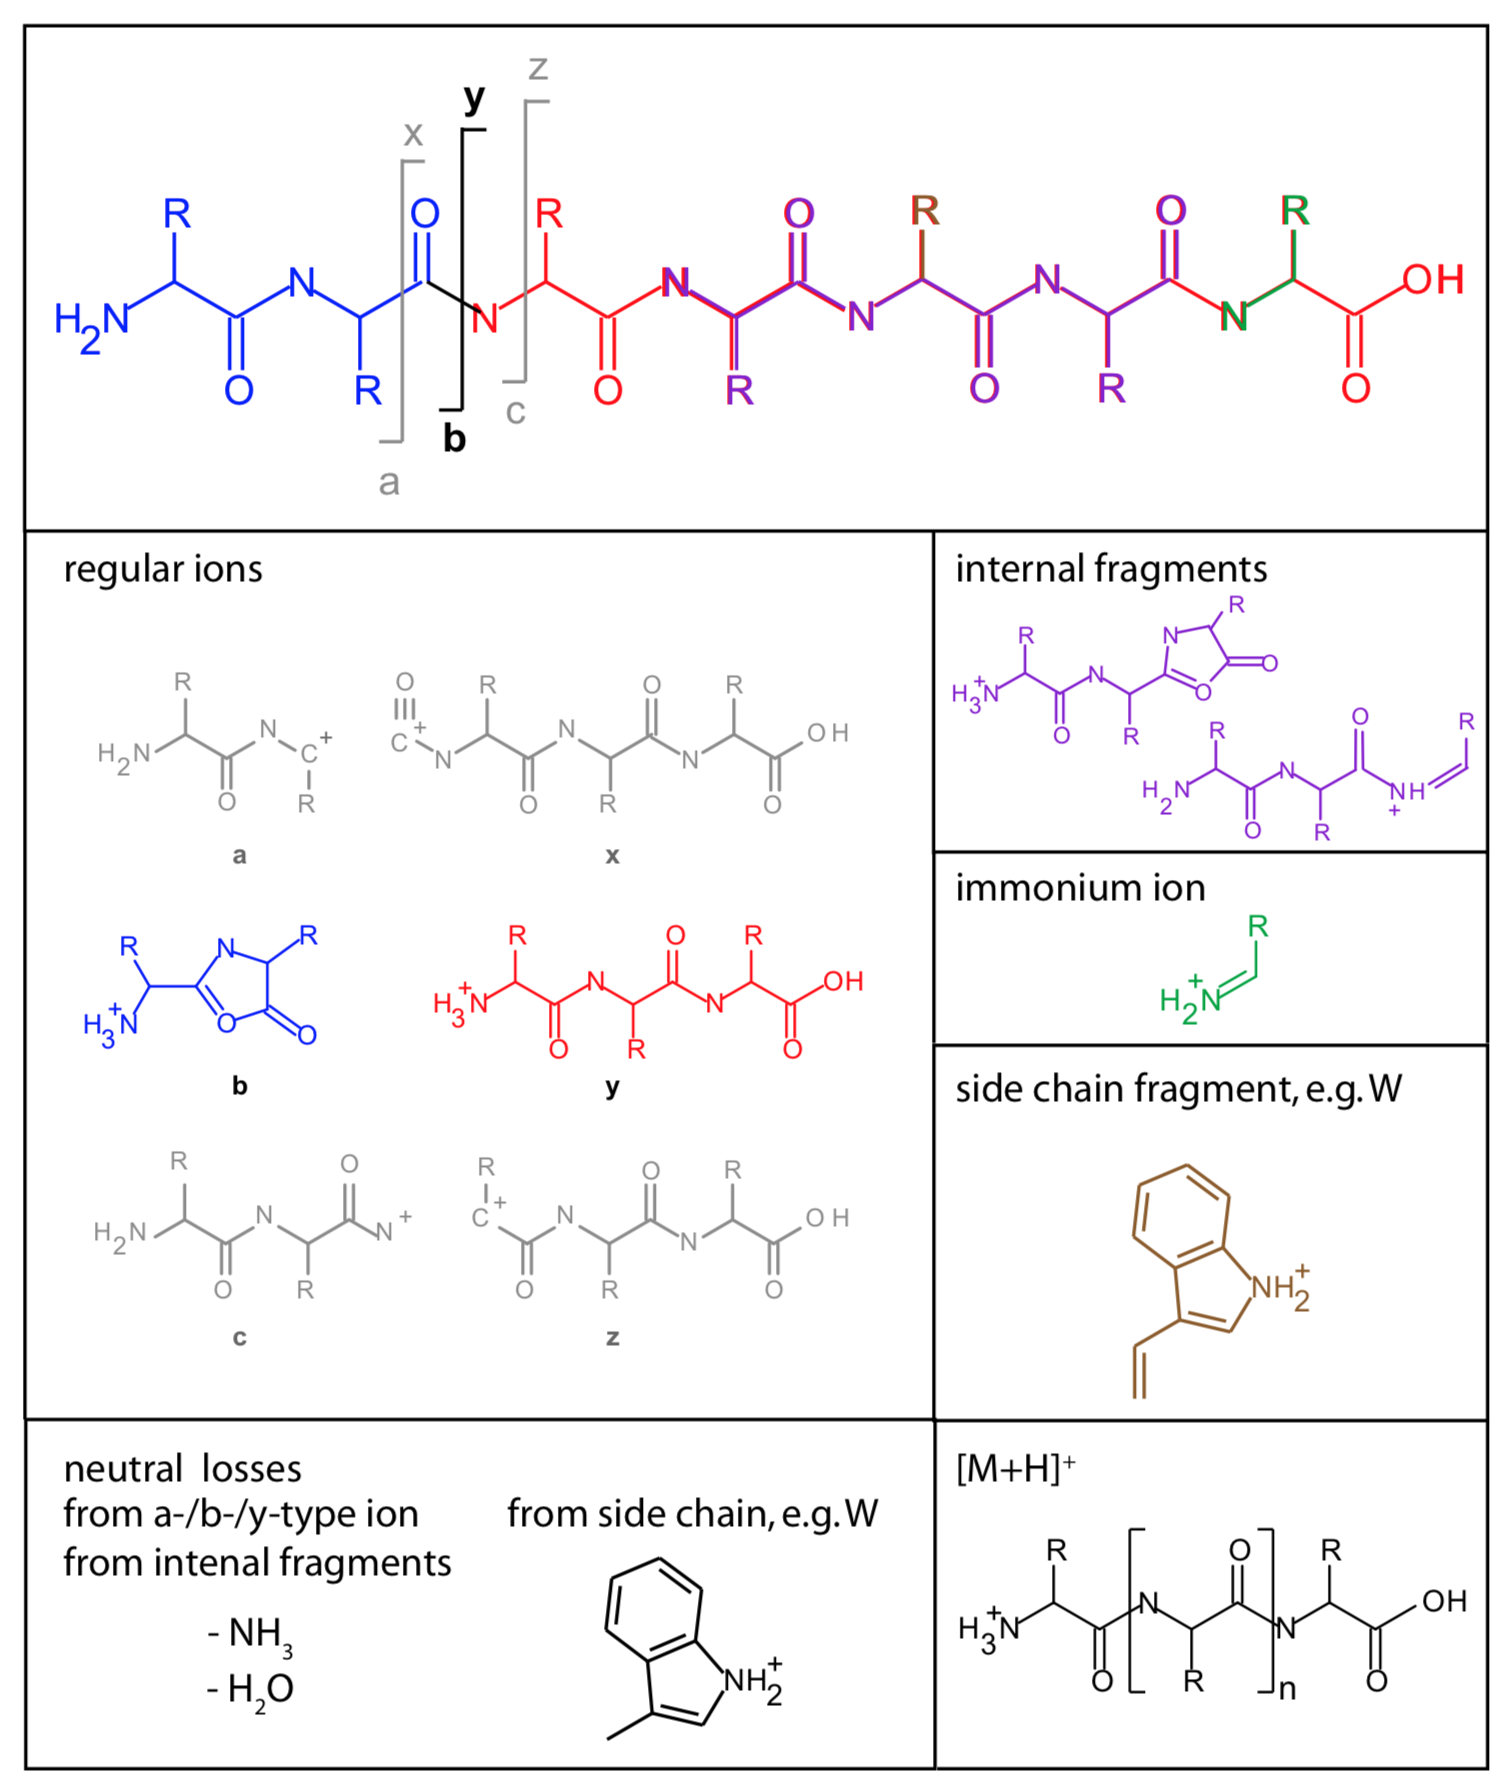
\includegraphics[width=.9\linewidth]{img/fragment-types-hcd.png}
  \caption{During HCD, \(b, y\), and to a lesser extent \(a\), ions are the most common, together with internal ions and immonium ions, and their counterparts with neutral losses. Image by~\citet{michalski2012systematic}.}\label{fig:fragment-types-hcd}
\end{figure}

\begin{figure}
  \centering
  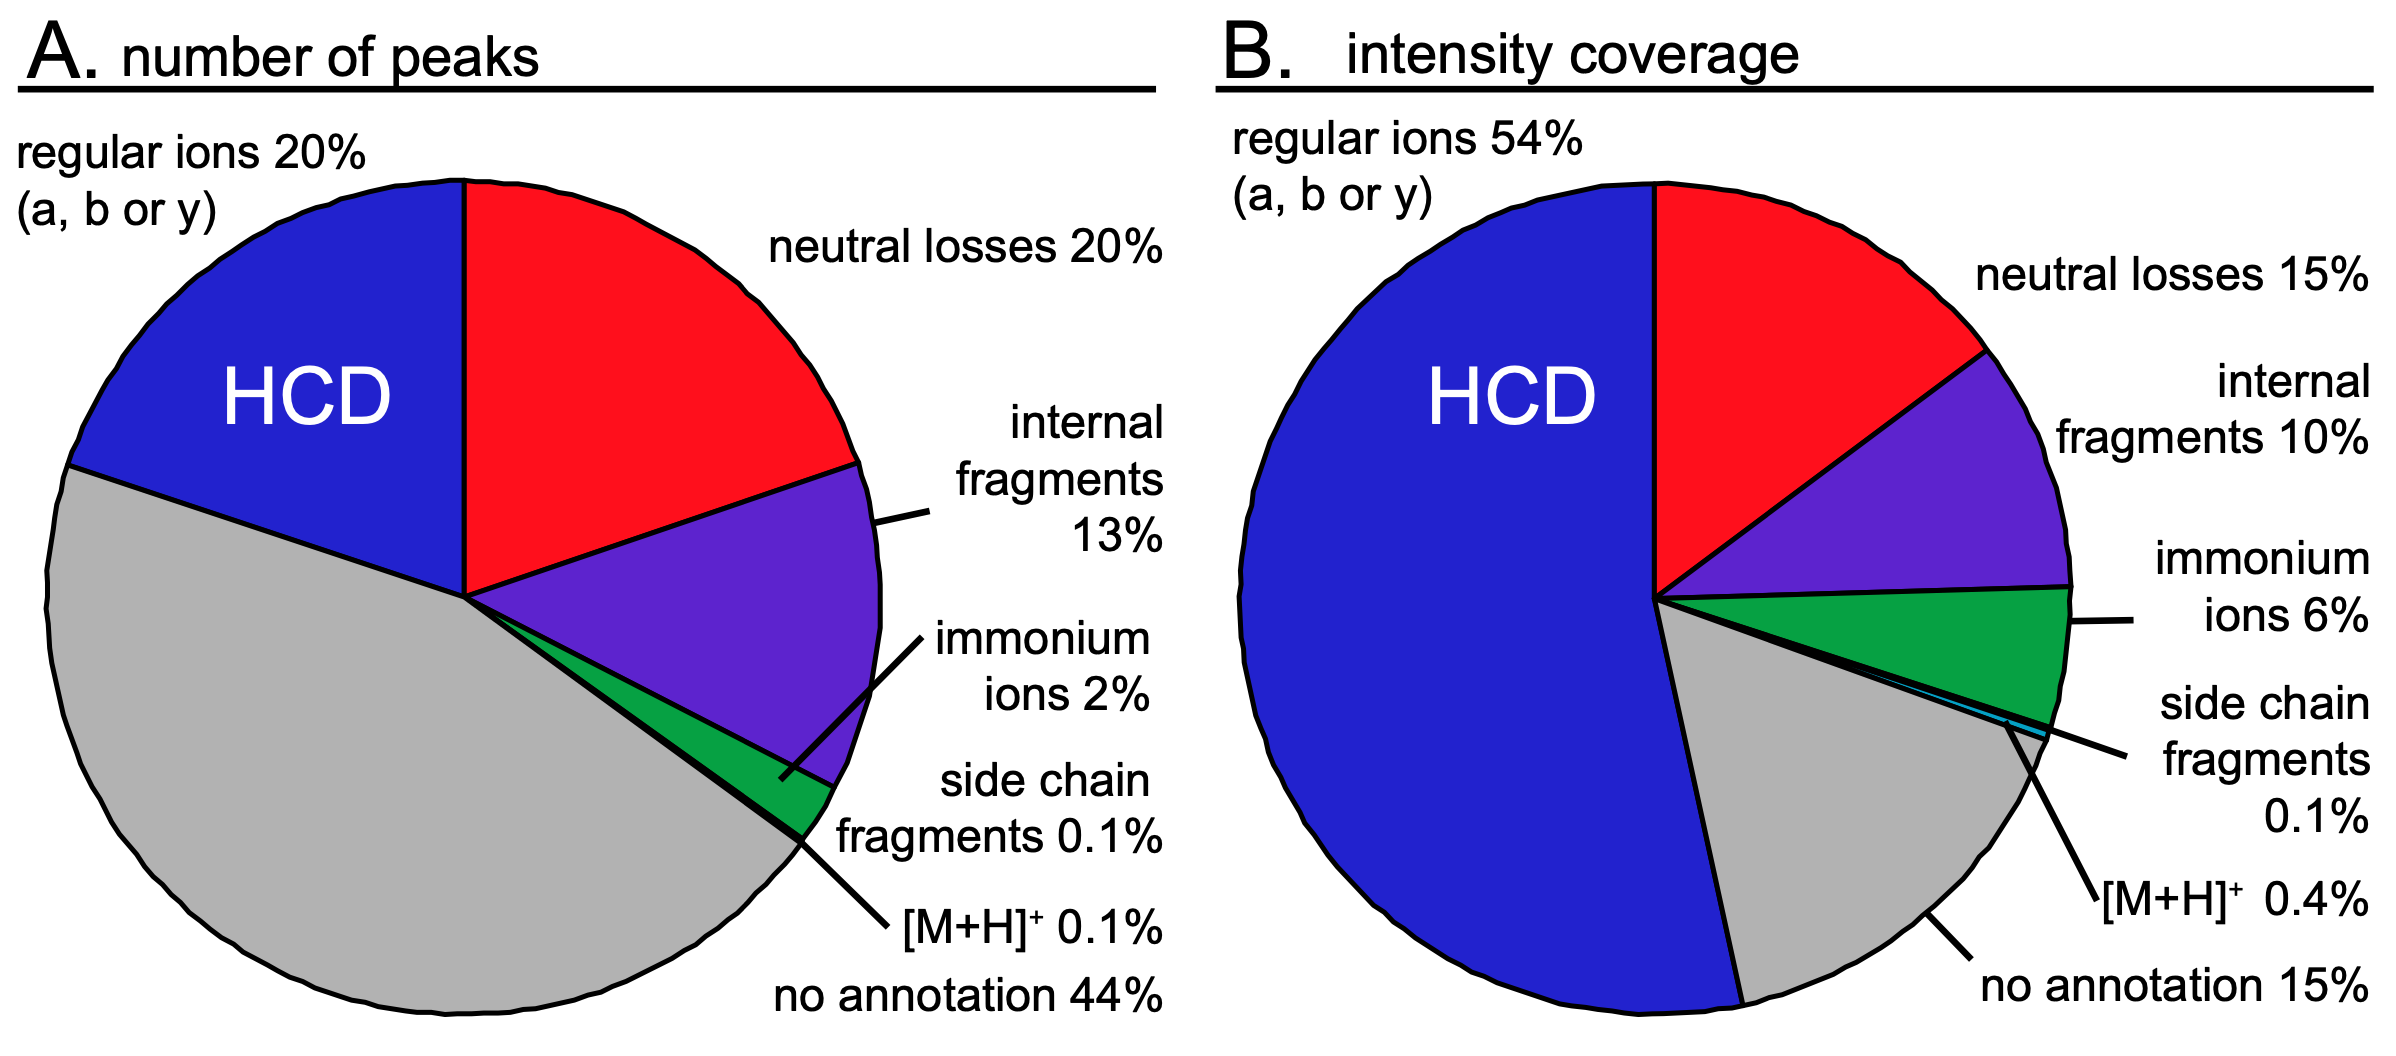
\includegraphics[width=.9\linewidth]{img/hcd.png}
  \caption{(B) The regular \(b, y\), and \(a\) ions take up 54\% of the measured spectral intensity. Another 25\% is explained by fragments with neutral-loss and internal fragments, and another 6\% by immonium ions. Together, those four account for 85\% of the measured intensity. It is true that almost a half of the peaks are still left unexplained (A), however, given all of these fragments have to split the remaining 15\% of intensity, they are probably rather rare and are only of moderate importance. Image by~\citet{michalski2012systematic}.}\label{fig:hcd}
\end{figure}

Although DBs are not affected by low-energy CID as much as the other PTMs~\cite{paizs2005fragmentation, lioe2007novel}, in high energy collision fragmentation such as HCD, cleavage of the S-S bond can be observed with a higher probability~\cite{bean1992characterization}. The cleavage of the bond can result in the formation of an asymetrical distribution of mass on the two cysteines~\cite{zhang2006mapping}, see \Cref{fig:disulfide-bond-cleavage-assymetry} for details. Additionally, the sole presence of a DB influences the fragmentation pathways of the whole peptide; \citet{mormann2008fragmentation} reports a low but detectable signal of peptide backbone cleavages in the bonds instide S-S loop of an internal DB, while \citet{clark2011collision} reports a higher frequence of internal ions.

\begin{figure}
  \centering
  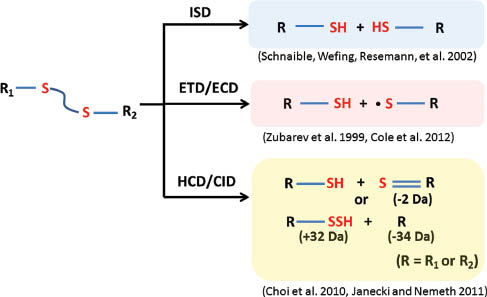
\includegraphics[width=.6\linewidth]{img/disulfide-bond-cleavage-assymetry.jpg}
  \caption{Under different dissociation strategies, DBs manifest different cleavage characteristics. Under CID, the cleavage results into two possible assymetrical mass distributions. Image by~\citet{tsai2013mass}.}\label{fig:disulfide-bond-cleavage-assymetry}
\end{figure}

To recapitulate, in theory a \(b\), \(y\), \(a\), or an internal ion can be seen in a HCD fragmentation spectra with zero or more of the following modifications:

\begin{enumerate}
  \item Dissociated neutral loss.
  \item Covalent modifications on some of the amino acid residues, such as methionine oxidation. A subset of these are the cysteine alkylations.
  \item A piece of a former DB that has been cleaved during the fragmentation.
  \item One or more fragments, possibly modified with some of the above, connected by a set of DBs. For some examples of crossliked fragments, see \Cref{fig:intrapeptide-bonds}.
\end{enumerate}

\begin{figure}
  \centering
  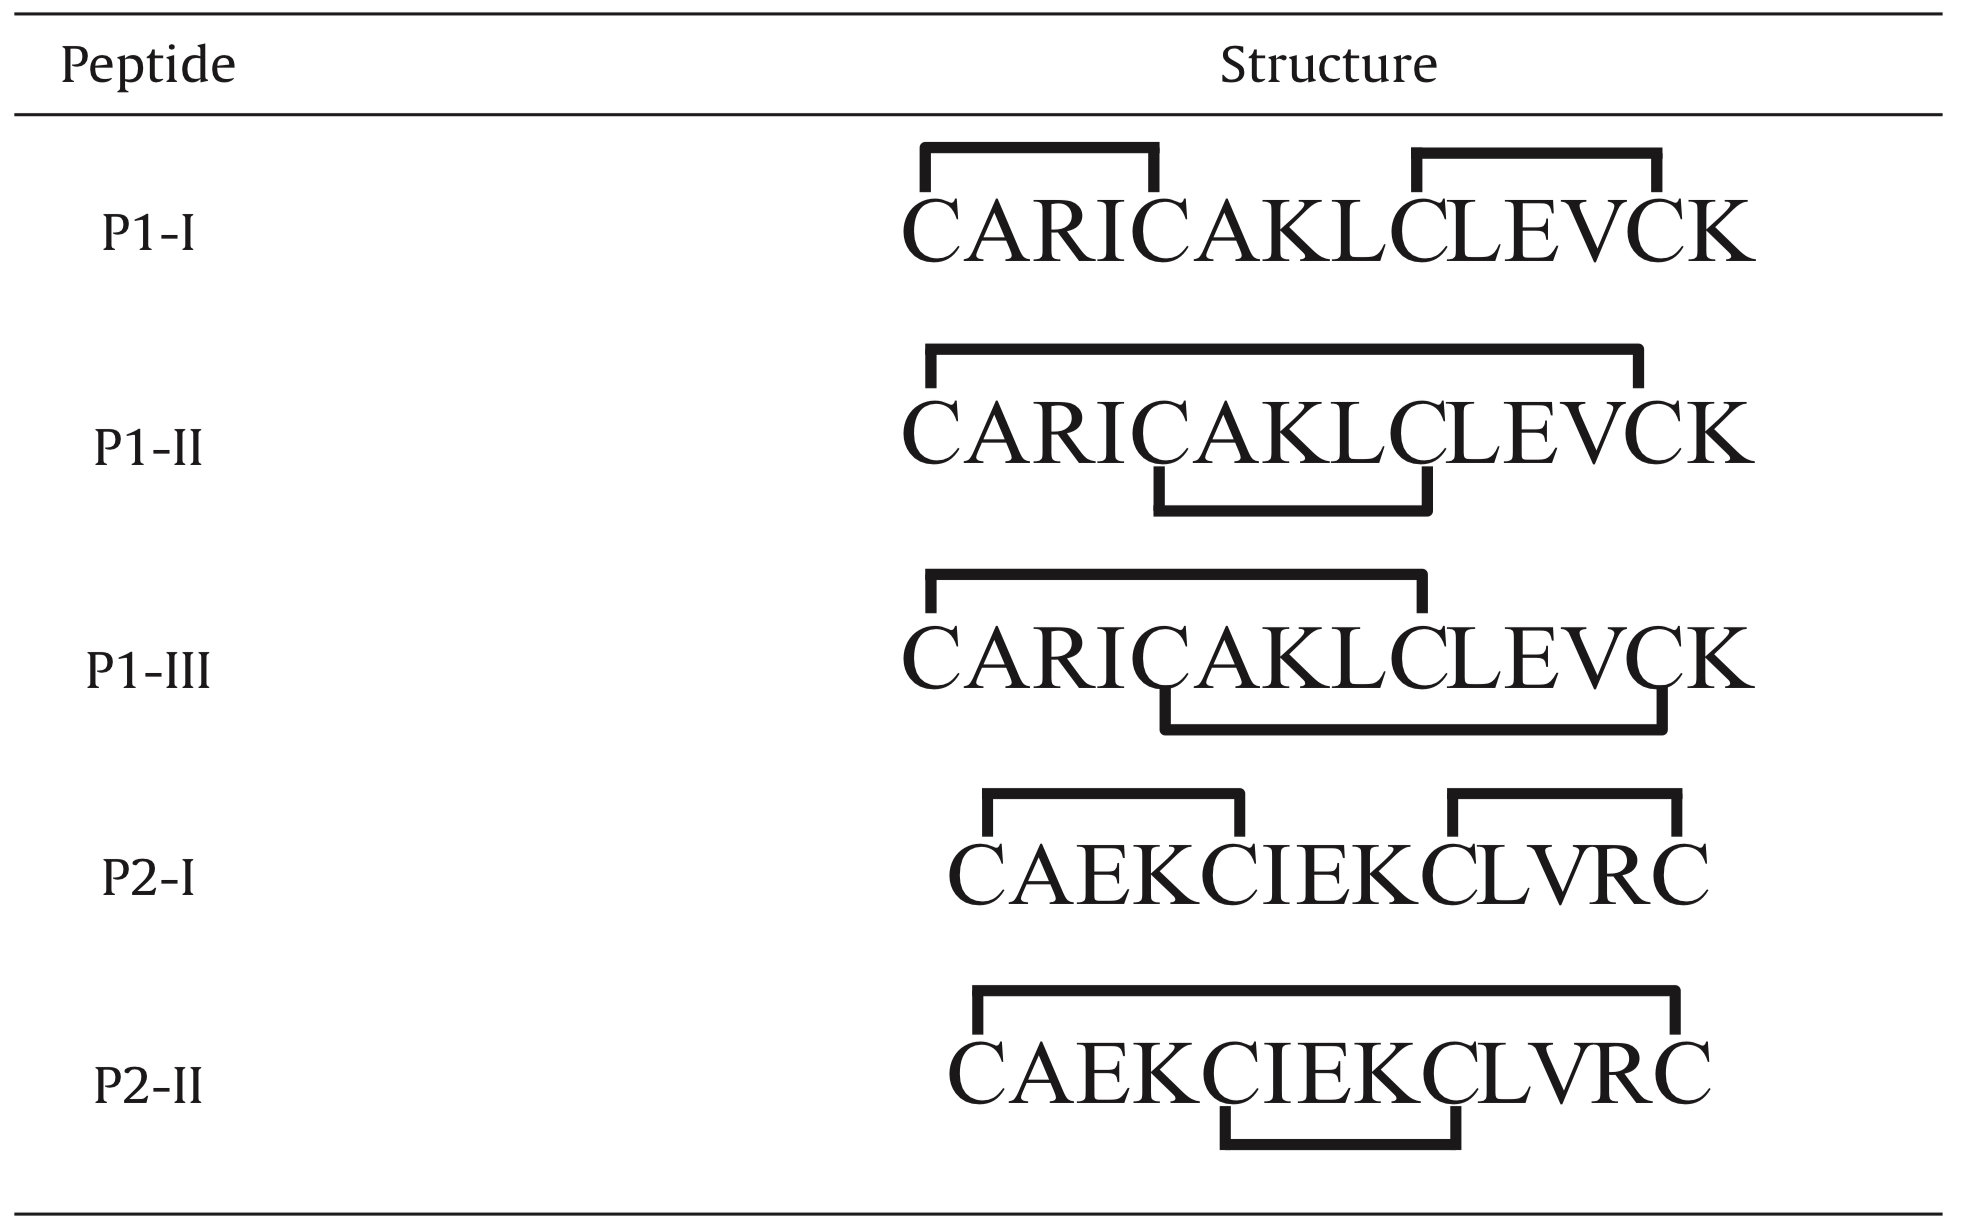
\includegraphics[width=.5\linewidth]{img/intrapeptide-bond.jpeg}
  \caption{An example of different possible configurations of intra-peptide DBs. Image by~\citet{durand2013tandem}.}\label{fig:intrapeptide-bonds}
\end{figure}

If we managed to identify the crosslinked fragments (category 4) in the measured data, we would gain a lot of important evidence about the presence of certain DBs in the protein. However, due to the complexity of the potential fragments, the fragment identification proces is very hard to automate completely. The next section details some of the current approaches to fragment assignment and DB mapping.

\section{Interpretation of fragmentation spectra from crosslinked peptides}\label{sec:analysis}

This section concerns itself with the existing methods that aim to determine the position of DBs in a protein using MS/MS data. After a short review of the manual and computation approaches to this problem, we formulate the task that this thesis is trying to solve in more precise terms, and finally perform a simple complexity analysis of the problem.

As noted by \citet{lakbub2018recent}, there are two main types of DB characterization.

\begin{itemize}
  \item Profile comparison methods make use of two samples: one reduced with the DBs removed, and one nonreduced whose DBs are still intact. Differential analysis is then deployed on a chromatogram profile of these two samples to determine which peptides are in the nonreduced sample, but not in the reduced one. Those peptides are suspect of containing DBs and are further analyzed in MS/MS\@.
  \item Intact analysis methods only use data from the nonreduced sample. Thus, they are simpler from the sample preparation standpoint, but have less information at their disposal than the profile comparison methods.
\end{itemize}

In each of the both categories, the protocols further differ in the choice of of sample separation, ionization, and fragmentation methods, the choice of mass analyzer, and whether the bulk of the analysis is performed manually or automatically~\cite{lakbub2018recent}. Some of the software for automatic DB characterisation is reviewd below; for the sake of completness, an example of a partially-manual method now follows.

\citet{wu2009mass} propose an intact analysis method based on LC-MS/MS with ETD\@. The prepared peptides are measured on MS\textsuperscript{1}, and fragmented by ETD\@. As described earlier, if the precursor ion contains DBs, they are dissociated in ETD, resulting in fragmentation spectra with two prominent peaks. The two peaks represent the two peptides that were connected by a DB to become the original precursor ion. Fragments from these two peaks are put into an MS\textsuperscript{3} step that employs CID fragmentation to acquire their sequence information. This sidesteps the problem of not having data from the non-bound peptides in the intact methods. Software for fragment mass searching and matching is used, but because it is not made with DB research in mind, the method requires frequent manual interventions.

It is clear that using specialised software for DB mapping would be preferable in this scenario. We reviewed some of the current computational methods in the next section.

\subsection{Current computational approaches}

Dedicated DB characterisation software usually only needs data from nonreduced samples. Nonetheless there are some commercial options that offer the possibility to add data from reduced samples, too, such as PepFinder and BioPharma Finder, as noted by \citet{lakbub2018recent}. The same authors offer a comprehensive list of past and current manual and compuational DB characterisation methods.

SimXL is tool for general peptide cross-linking analysis~\cite{lima2015sim}, including DBs~\cite{cui2019comprehensive}. SimXL has three main differentiating factors. Frist is the user-friendly UI that allows the reasearchers to view not only the interpreted results, but also the annotated data based on which they were computed. Second is its search space reduction heuristic based on the presence of a reporter ion~\cite{iglesias2010identification}, a peak that is specific to the fragmentation spectra of a crosslinked precursor. Finally, SimXL employs a further search space-reduction heuristic based on dead-end modifications, but we believe it is probably inapplicable in the context of DB characterisation.

A popular method by \citet{liu2014facilitating} includes a recommened research protocol, starting with protein digestion. Samples are digested with pepsin to avoid DB scrambling, fragmented with ETD followed by HCD, or (EThcD) for short, and finally analyzed with SlinkS, a dedicated DB matching algorithm. As mentioned previously, it is possible to extract information about the peptides constituting the precursor ion from the ETD fragmentation spectra. The HCD step is employed in order to gain sequence information about these peptides, similary to how MS\textsuperscript{3} has been used in~\cite{wu2009mass}.

Ultimately, thanks to EThcD, two peaks corresponding to the precursor peptide pair are identified in each fragmentation spectrum. Aditionally, the whole precursor match is scored by scoring the fragments, now that it is known from which precursor they (allegedly) originated. The main shortcoming of this method is the fact that it only works with dipeptide precursors connected by a single DB; it also ignores fragments with neutral loss and internal ion fragments. That makes it impossible to identify some of the more complicated DB configurations, such as the ones on \Cref{fig:intrapeptide-bonds}.

In fact, all of the aforemetioned methods should be able to match simple interpeptide DBs, but they reportedly struggle with more complex DB configurations~\cite{lakbub2018recent}; for some examples of complicated DB configurations, see \Cref{fig:bond-types}.

A wide array of approaches to DBs is offered, leading to a yet wider array of recommended sample preparation and fragmentaion protocols. We conclude that computational DB characterisation is a hard problem to solve, a notion we formalize in the next section.

\begin{figure}
  \centering
  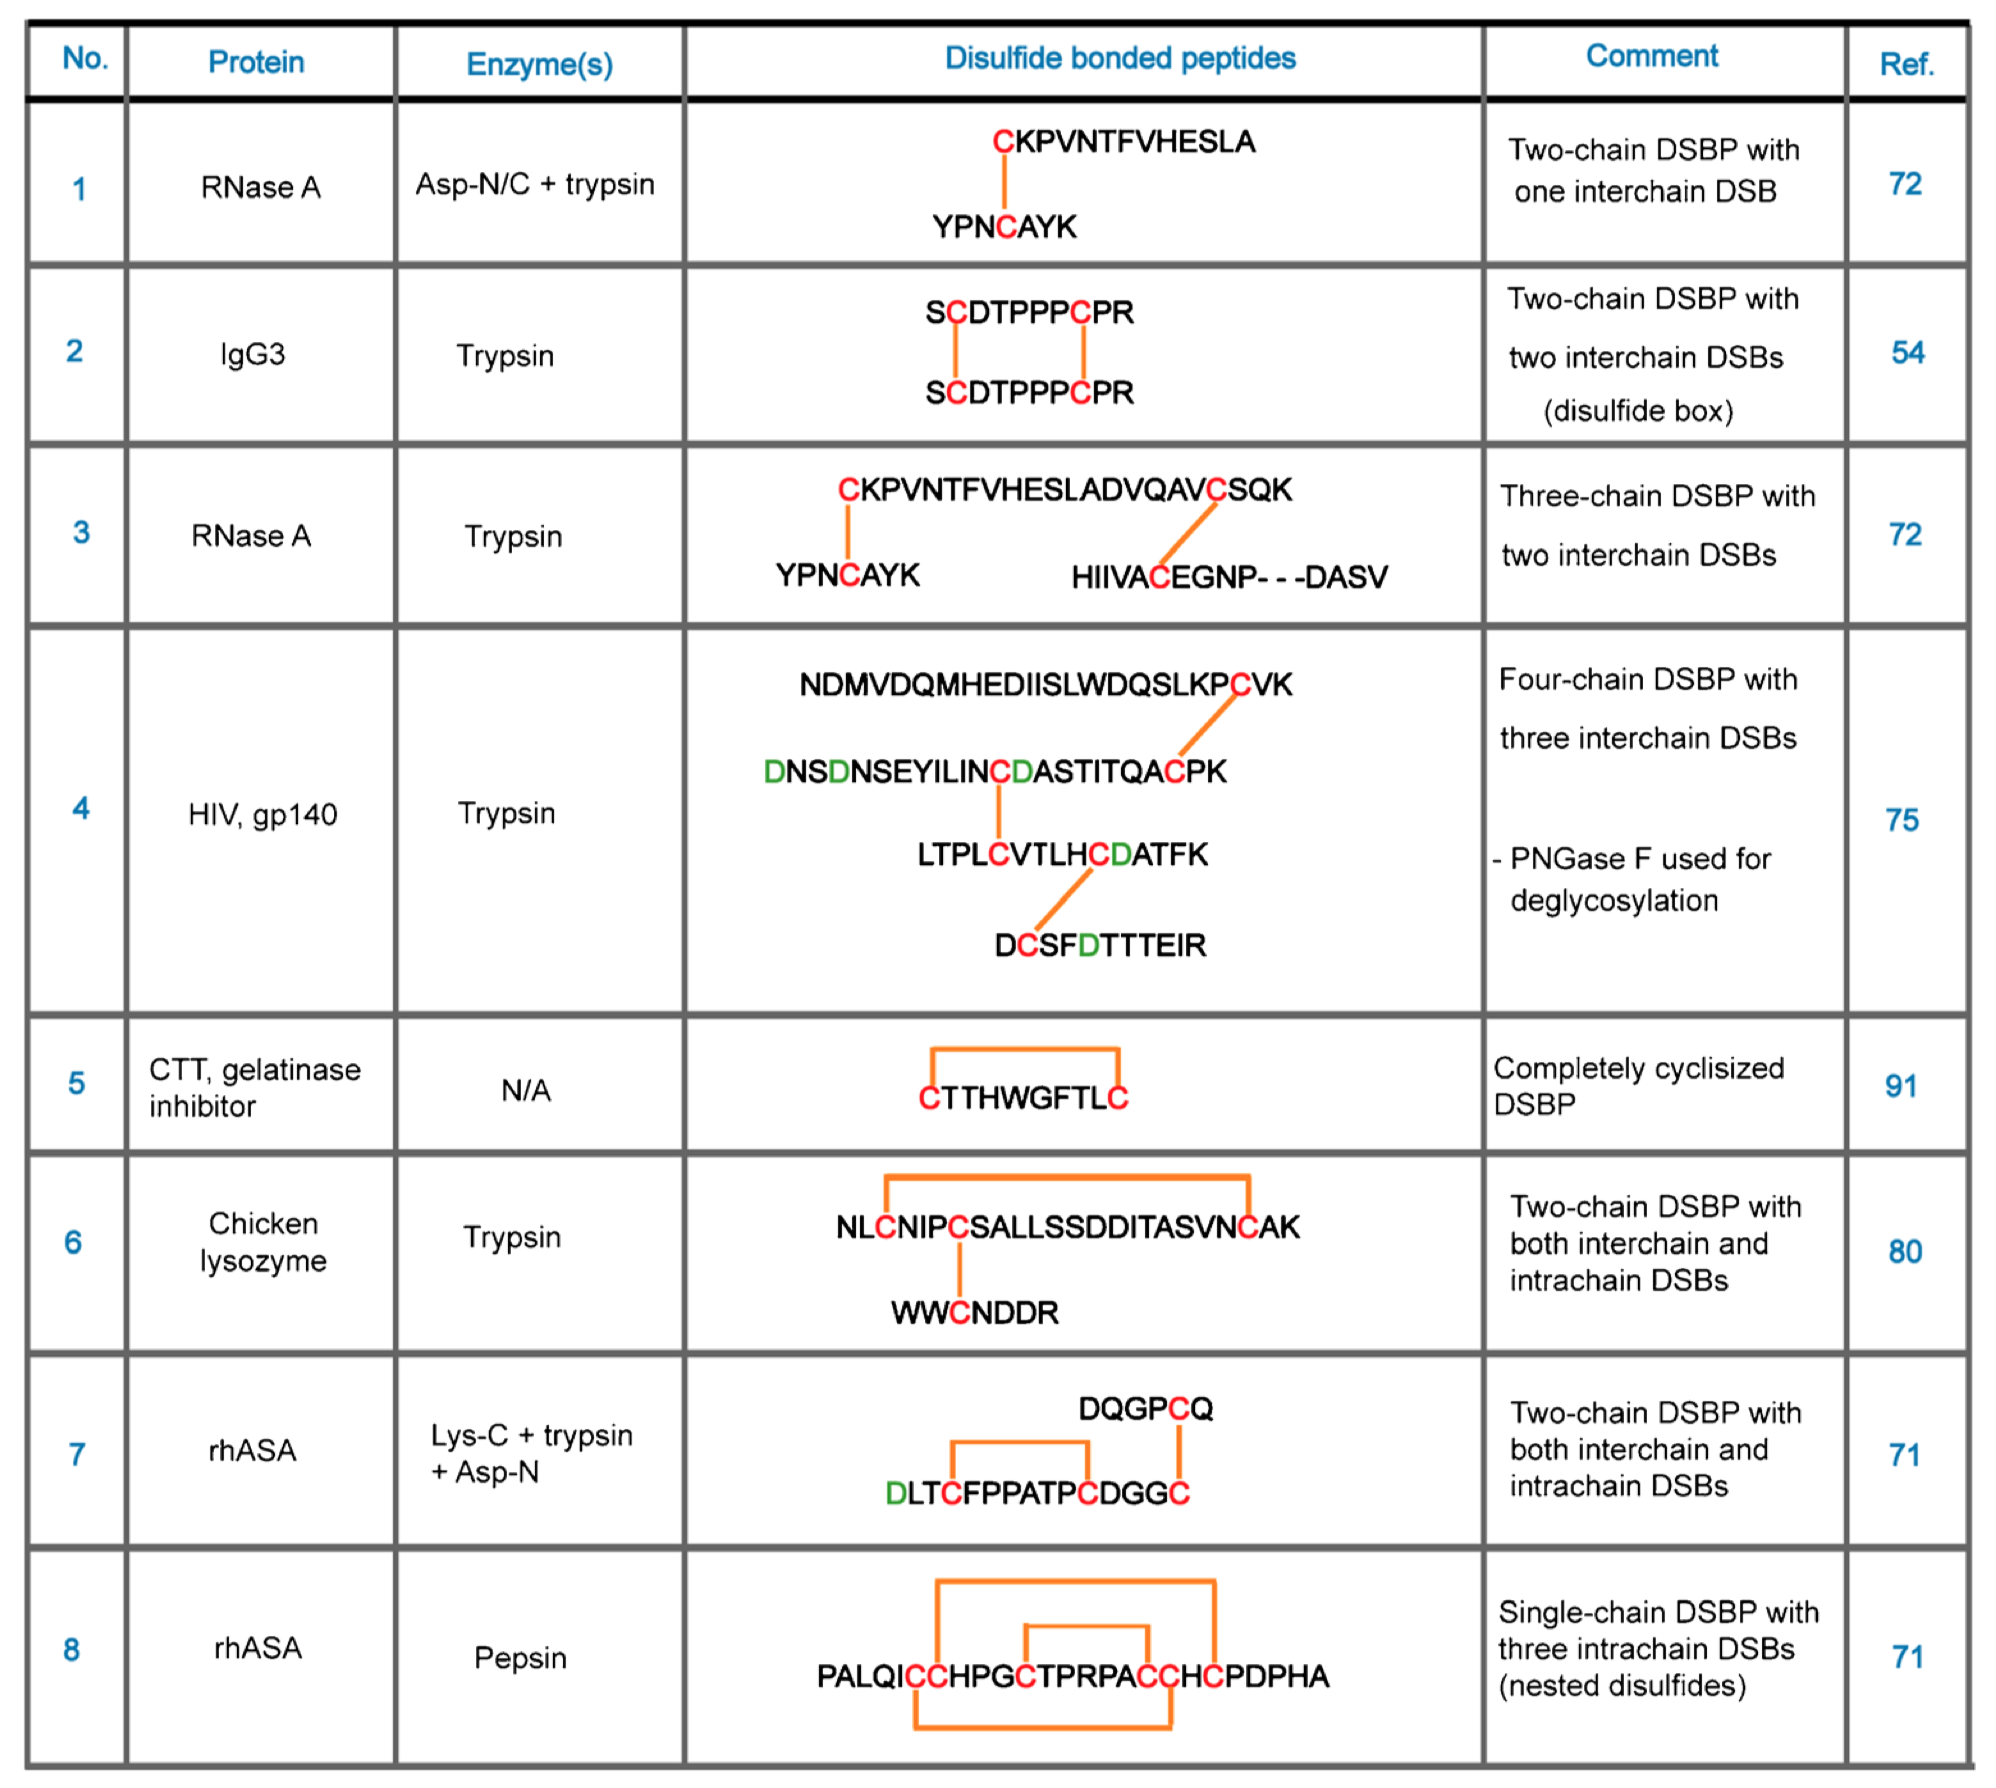
\includegraphics[width=1\linewidth]{img/bond-types.png}
  \caption{Illustrative examles of different ways peptides can be connected by disulfide bonds, ranging from realtively simple examples (1, 3, 5) to complex multipeptide or multibond configurations (4, 8). The more complicated configurations proved to be hard to characterise computationally. Image by~\citet{lakbub2018recent}. (DSB = disulfide bond, gp140 = glycoprotein 140, rhASA = recombinant human arylsulfatase A)}\label{fig:bond-types}
\end{figure}


\subsection{Computational complexity of crosslinked fragment identification}

Undisputably, the problem of determining the characteristics of DB linkages in proteins is hard. From biochemical point of view, already sample preparation poses a challenge; there is a need to minimize DB scrambling, but at the same time have the protease be as specific as possible to simplify the subseqeucnt analysis.

Another unresolved problem is the choice of dissociation method. ETD spectra offer the information about the constituent peptides, which is useful when assigning precursor peptides. On the other hand, CID-based approaches have access to richer but more complicated fragmentation spectra, including interlinked fragments and internal ions with intact DBs; these are useful for precise pinpointing of the DB location.

To continue this discussion further, we need to be specific about the precise task we are attempting to solve. The ultimate goal is to determine where all DBs in a protein are located, even if they are in complex configurations. In this thesis, we try to reach this goal by identifying a wide array of fragments in the measured fragmentation spectra, and aggregating the evidence they provide about positions of the individual DBs. So, to solve the original DB mapping problem, we need to be able to identify even complex fragments in MS/MS data.

\subsubsection{A formalised perspective of the task}

We have a known precursor with defined DB positions, that we will call a \emph{variant}, and a measured fragmentation spectrum. Our task is to say how well the variant matches the spectrum, by trying to assign in-silico generated fragments of the variant to the different measured peaks. Mathematically, we can represent the variant by a \emph{variant graph}.

\begin{defn}
  A \emph{variant graph} of a variant \(R\) comprising of \(n\) residues is a graph \(G_R = (V, E)\) with weighted nodes, where \(V  = 1\ldots n\) and \((i, j) \in E\) if and only if there is a peptide or a disulfide bond connecting  the \(i\)-th and \(j\)-th residue in \(R\). The weight \(w_i\) of the vertex \(i\) is the mass of the corresponding \(i\)-th residue in the precursor.
\end{defn}

Even though the bonds in \(R\) are constrained in terms of connectivity --- there can be at most one DB connected to a given residue, and at most two peptide bonds --- \(G_R\) can still in theory be a relatively complex non-planar graph, as illustrated on \Cref{fig:nonplanar}.

\begin{figure}
  \centering
  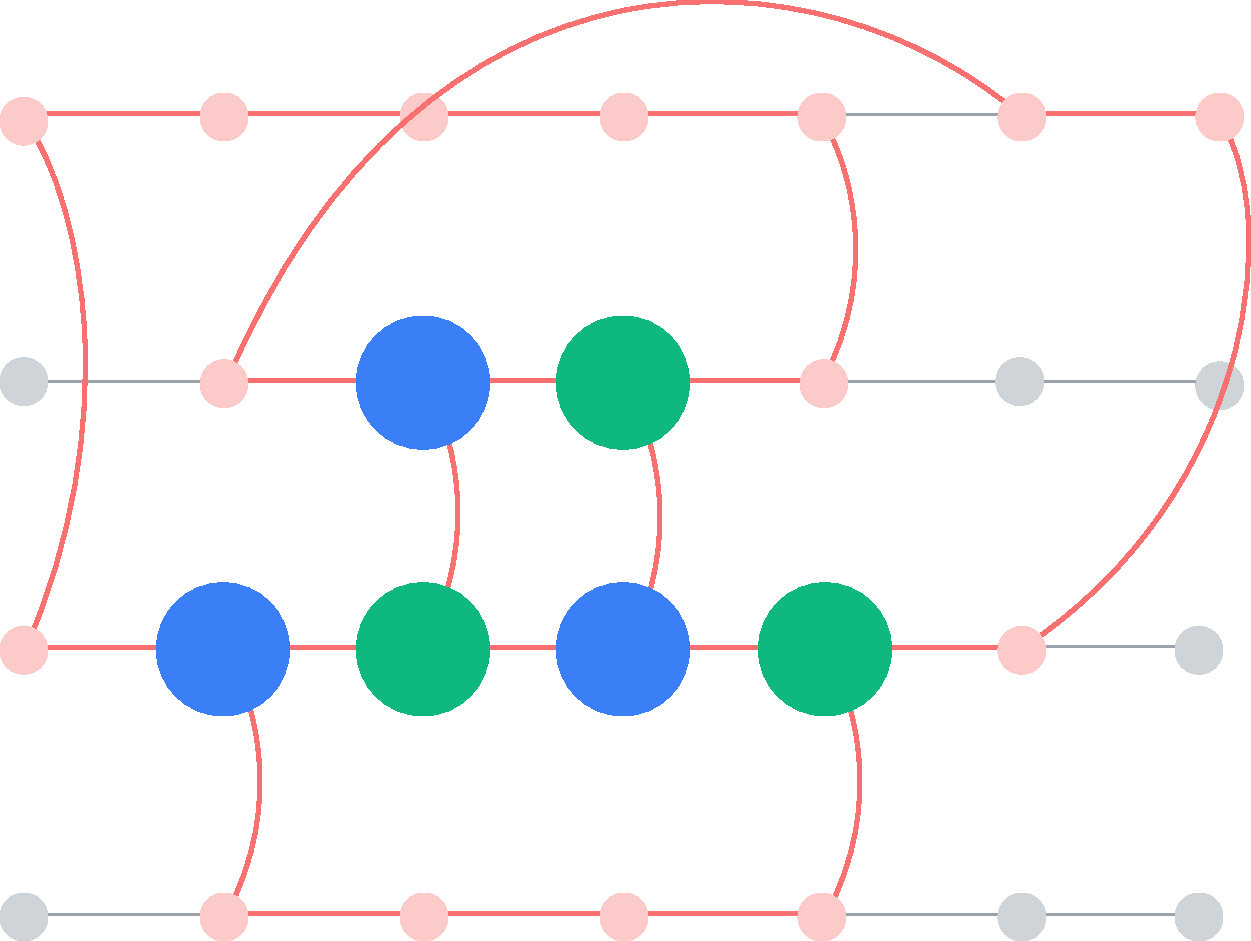
\includegraphics[width=0.5\linewidth]{img/nonplanar.pdf}
  \caption{An example of a valid precursor graph that is not planar due to the presence of a \(K_{3, 3}\) subdivision~\cite{kuratowski1930probleme} (highlighted). Vertices represent amino acid residues, horizontal lines represent peptide bonds, and vertical curved lines represent disulfide bonds. The precursor could be made out of four different interlinked peptides, but it is alsopossible for it to be a single peptide with many intrapeptide disulfide bonds.}\label{fig:nonplanar}
\end{figure}

\begin{lemma}\label{lemma:fragment}
  Every fragment \(A\) of the variant \(R\) can be represented as a connected weighted subgraph in \(G_R\), and every connected subgraph in \(G_R\) represents a fragment of \(R\). We will denote the connected subgraph represeting the fragment \(A\) as \(F_A\).
\end{lemma}

\begin{lemma}\label{lemma:mass}
  The number of cleavages that were required to create the fragment \(A\) is equal to the number of edges that have at least one vertex in \(F_A\), but are not themselves in its set of edges. The mass of \(A\) can be computed by summing up the weights of its vertices \(F_A\).
\end{lemma}

The task of matching the whole variant to a spectrum can be split into multiple subtasks of trying to find a fragment of the variant that matches a mass of a specific peak. By using \Cref{lemma:fragment} and \Cref{lemma:mass} we can reformulate the subtask as searching for a connected subgraph in \(G_R\) in which the sum of vertex weights is equal to the mass of the peak we are trying to match. This problem is usually called the exact weight subraph problem~\cite{abboud2013exact}, or, in our case, an exact weight \emph{connected} subgraph problem.

A well-studied closely related problem called the maximum weight connected k-subgraph problem was shown to be NP-hard on general graphs, and even on planar and bipartite graphs with integer weights~\cite{hochbaum1994node}.\footnote{The same authors propose a polynomial-time \(O(k^2n)\) dynamic programming algorithm for a restricted version of the problem searching for subgraphs in trees.} The exact weight connected subgraph problem has not been studied quite as thoroughly, but we believe it is safe to assume that its complexity will not be much lower. In other words, in the context of our not-necessarily-planar precursor graphs, the problem is likely NP-hard.

Furthermore, this was only a simplified look on the fragment matching problem. In reality, we are not looking for an exact match, but we have a tolerance range whose size is not absolute, but is defined relative to the mass of the generated fragment (in ppm). We also have to take into account the possible modifications of amino acid residues, the possibile occurences of a neutral loss, and the asymetrical nature of disulfide bond cleavage under CID, adding additional complexity to an already complex problem.

Nevertheless, in the next chapter we describe a general algorithm that attempts to solve the fragment matching problem, and use the results to identify DBs in the original protein. We apply an upper bound on the number of cleavages of matched fragments, which limits the search space considerably. We also employ strict limits regarding the matching error, which enables us to search the space in a branch-and-bound fashion.

% \chapter{Important first chapter}
% \label{chap:refs}

% First chapter usually builds the theoretical background necessary for readers to understand the rest of the thesis. You should summarize and reference a lot of existing literature and research.

% You should use the standard \emph{citations}\todo{Use \textbackslash{}emph command like this, to highlight the first occurrence of an important word or term. Reader will notice it, and hopefully remember the importance.}.

% \begin{description}
% \item[Obtaining bibTeX citation] Go to Google Scholar\footnote{\url{https://scholar.google.com}}\todo{This footnote is an acceptable way to `cite' webpages or URLs. Documents without proper titles, authors and publishers generally do not form citations. For this reason, avoid citations of wikipedia pages.}, find the relevant literature, click the tiny double-quote button below the link, and copy the bibTeX entry.
% \item[Saving the citation] Insert the bibTeX entry to the file \texttt{refs.bib}. On the first line of the entry you should see the short reference name --- from Scholar, it usually looks like \texttt{author2015title} --- you will use that to refer to the citation.
% \item[Using the citation] Use the \verb|\cite| command to typeset the citation number correctly in the text; a long citation description will be automaticaly added to the bibliography at the end of the thesis. Always use a non-breakable space before the citing parenthesis to avoid unacceptable line breaks:
% \begin{Verbatim}
% Trees utilize gravity to invade ye
% noble sires~\cite{newton1666apple}.
% \end{Verbatim}
% \item[Why should I bother with citations at all?] For two main reasons:
% \begin{itemize}
% \item You do not have to explain everything in the thesis; instead you send the reader to refer to details in some other literature. Use citations to simplify the detailed explanations.
% \item If you describe something that already exists without using a citation, the reviewer may think that you \emph{claim} to have invented it. Expectably, he will demand academic correctness, and, from your perspective, being accused of plagiarism is not a good starting point for a successful defense. Use citations to identify the people who invented the ideas that you build upon.
% \end{itemize}
% \item[How many citations should I use?]
% Cite any non-trivial building block or assumption that you use, if it is published in the literature. You do not have to cite trivia, such as the basic definitions taught in the introductory courses.

% The rule of thumb is that you should read, understand and briefly review at least around 4 scientific papers. A thesis that contains less than 3 sound citations will spark doubt in reviewers.
% \end{description}

% There are several main commands for inserting citations, used as follows:
% \begin{itemize}
% \item \citet{knuth1979tex} described a great system for typesetting theses.
% \item We are typesetting this thesis with \LaTeX, which is based on \TeX{} and METAFONT~\cite{knuth1979tex}.
% \item \TeX{} was expanded to \LaTeX{} by \citet{lamport1994latex}, hence the name.
% \item Revered are the authors of these systems!~\cite{knuth1979tex,lamport1994latex}
% \end{itemize}

% \section{Some extra assorted hints before you start writing English}

% Strictly adhere to the English word order rules. The sentences follow a fixed structure with subject followed by a verb and an object (in this order). Exceptions to this rule must be handled specially, and usually separated by commas.


% Mind the rules for placing commas:
% \begin{itemize}
% \item Use the \emph{Oxford comma} before `and' and `or' at the end of a longer, comma-separated list of items. Certainly use it to disambiguate any possible mixtures of conjunctions: \textit{`The car is available in red, red and green, and green versions.'}
% \item Do not use the comma before subordinate clauses that begin with `that' (like this one). English does not use subordinate clauses as often as Slavic languages because the lack of a suitable word inflection method makes them hard to understand. In scientific English, try to avoid them as much as possible. Ask doubtfully whether each `which' and `when' is necessary --- most of these helper conjunctions can be removed by converting the clause to non-subordinate.

% As an usual example, \xxx{\textit{`The sentence, which I wrote, seemed ugly.'}} is perfectly bad; slightly improved by \xxx{\textit{`The sentence that I wrote seemed ugly.'}}, which can be easily reduced to \textit{`The sentence I wrote seemed ugly.'}. A final version with added storytelling value could say \textit{`I wrote a sentence but it seemed ugly.'}
% \item Consider placing extra commas around any parts of the sentence that break the usual word order, especially if they are longer than a single word.
% \end{itemize}

% Do not write long sentences. One sentence should contain exactly one fact. Multiple facts should be grouped in a paragraph to communicate one coherent idea. Paragraphs are grouped in labeled sections for a sole purpose of making the navigation in the thesis easier. Do not use the headings as `names for paragraphs' --- the text should make perfect sense even if all headings are removed. If a section of your text contains one paragraph per heading, you might have wanted to write an explicit list instead.

% Every noun needs a determiner (`a', `the', `my', `some', \dots); the exceptions to this rule, such as non-adjectivized names and indeterminate plural, are relatively scarce. Without a determiner, a noun can be easily mistaken for something completely different, such as an adjective or a verb.

% Consult the books by \citet{glasman2010science} and \citet{sparling1989english} for more useful details.
